\documentclass{article}

\setlength{\parindent}{0pt}
\usepackage{cite}
\usepackage{tikz}
\newcommand\independent{\protect\mathpalette{\protect\independenT}{\perp}}
\def\independenT#1#2{\mathrel{\rlap{$#1#2$}\mkern2mu{#1#2}}}
\begin{document}
\section{Implementation}
\subsection{Skeleton}
\subsubsection{Indpendence Test}
The first sprint consisted of implementing the PC algorithm. This began with implementing a function to determine the skeleton of the graph. To estimate the skeleton a function to determine independence and conditional independence of data was needed. The chi squared tests for independence and conditional independence were chosen. This test will only work on discrete data however other tests could be substituted for other data.
\\

Pandas dataframes were chosen to store data during the algorithm as they provide easy indexing and many useful functions. The crosstab function was especially useful when implementing the chi squared tests as it could automatically compute the contingency tables needed for the tests.
\\

A function prepare\_data was implemented to read data from a file into a data frame for processing.\\

The unconditional independence test was fairly straightforward to implement as it only consisted of computing the contingency tables and then comparing the values in the tables to the sums of the rows and columns in the tables.\\

The conditional case was more complex, first the conditioning set was combined into a single variable through concatenation of each variable in every data point. This made making a contingency table across all the observed values significantly easier. Next a contingency table across the three variables was needed. Again the cross tab function was used, however calculating the sums of each time a variable takes a particular value was now more complex, this is because the columns for the conditioning set were split between the columns for the Y variable.\\

On top of this not all values of Y and Z were observed simultaneously in data so
we cant simply iterate through all values of y and z and some up the associated columns as some do not exist. First the columns that exist must be found and then they can be summed over. After this the test is similar to the unconditional however the expected valued will now also account for the value of the conditioning set.
\\

The scipy chi2 function was then used to calculate the chi2 statistic and p-value which is returned by the function.\\

\subsubsection{Variables to be tested}
With this function the skeleton can be found. A fully connected networkx Graph is generated and then edges between nodes that show conditional independence are removed. 

First unconditional independence tests are performed between each pair of variables and edges removed between those that are found to be independent. The conditional tests based on variables adjacent to the first variable with size of the set increasing by one after all tests have been performed. When first implemented, the algorithm tested $X \independent Y | Z$ and $Y \independent X | Z$, this is inefficient as many tests are repeated. It is however not enough to simply test $X \independent Y | Z$ as the value of $Z$ is dependent on first variable. To avoid repeated tests, the test performed were stored and only performed if they did not exist in the store.\\

Edge orientation requires the separation set of each pair of variables. This was stored as a dictionary of all pairs of edges and simply updated with a conditioning set if that set was found to condition independence between the pair.\\

Since all of the algorithms learn a skeleton, the function is a method of the GraphLearner class which is the parent class of the other algorithm classes. The function returns a networkx Graph containing the estimated edges of the skeleton and a dictionary containing the separation set of each pair of variables.\\

\subsection{PC edge orientation}
For the pc algorithm edge orientation is relatively simple. However, the pc algorithm outputs a PDAG which contains a mixture of directed and undirected edges, networkx does not contain a data structure to support this kind of graph so one had to be implemented. This turned out to be fairly trivial, using a directed graph behind the scenes in which undirected edges were represented as bidirected edge. Since it's a DAG there cant be any actual bidirected edges so all bidirected edges can simply be considered to be undirected.\\

When finding the edges orientation, one graph was used to store directed and one used to store undirected. When an edge was directed it was simply transferred from one to the other and once all edges that can be oriented are oriented, the two graphs are combined into a PDAG.\\

\subsubsection{V-Structures}
The first part of edge orientation consists of identifying colliders. This is fairly simple as you simply need to find V structures and test if the node that is adjacent to two of the variables is in their separation set. If it is orient the edges toward that node.\\

However, there may be situations in which the order of the v-structures you test affects the final orientation of the graph. There may be two connected v-structures where orienting one will also orient the other but not in the direction described by the constraints.\\

\begin{center}
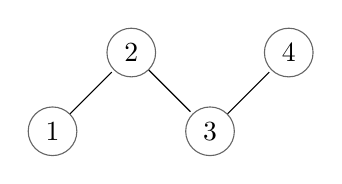
\begin{tikzpicture}[shorten >=1pt,->]
\tikzstyle{vertex}=[circle, draw=black!60, minimum size=12pt]
\node[vertex] (G_1) at (-1,-1) {1};
\node[vertex] (G_2) at (0,0)   {2};
\node[vertex] (G_3) at (1,-1)  {3};
\node[vertex] (G_4) at (2,0)  {4};
\draw [-] (G_1) -- (G_2);
\draw [-] (G_2) -- (G_3);
\draw [-] (G_3) -- (G_4);
\end{tikzpicture}
\end{center}



\begin{center}
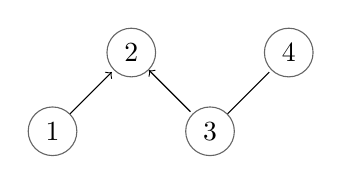
\begin{tikzpicture}[shorten >=1pt,->]
\tikzstyle{vertex}=[circle, draw=black!60, minimum size=12pt]
\node[vertex] (G_1) at (-1,-1) {1};
\node[vertex] (G_2) at (0,0)   {2};
\node[vertex] (G_3) at (1,-1)  {3};
\node[vertex] (G_4) at (2,0)  {4};
\draw [->] (G_1) -- (G_2);
\draw [<-] (G_2) -- (G_3);
\draw [-] (G_3) -- (G_4);
\end{tikzpicture}
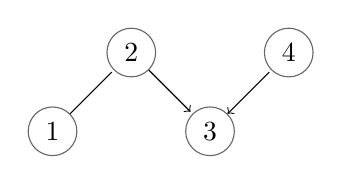
\begin{tikzpicture}[shorten >=1pt,->]
\tikzstyle{vertex}=[circle, draw=black!60, minimum size=12pt]
\node[vertex] (G_1) at (-1,-1) {1};
\node[vertex] (G_2) at (0,0)   {2};
\node[vertex] (G_3) at (1,-1)  {3};
\node[vertex] (G_4) at (2,0)  {4};
\draw [-] (G_1) -- (G_2);
\draw [->] (G_2) -- (G_3);
\draw [<-] (G_3) -- (G_4);
\end{tikzpicture}
\end{center}

Figure - shows two possible orientations, depending on which v structure is oriented first, in the first case when we arrive at the 2,3,4 triple one of two thing can be done. The edge (3,4) can be left undirected or the new structure can override the old one, as shown in figure - .\\

\begin{center}
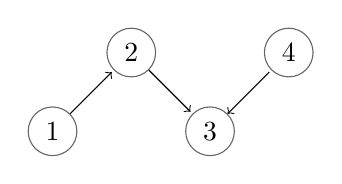
\begin{tikzpicture}[shorten >=1pt,->]
\tikzstyle{vertex}=[circle, draw=black!60, minimum size=12pt]
\node[vertex] (G_1) at (-1,-1) {1};
\node[vertex] (G_2) at (0,0)   {2};
\node[vertex] (G_3) at (1,-1)  {3};
\node[vertex] (G_4) at (2,0)  {4};
\draw [->] (G_1) -- (G_2);
\draw [->] (G_2) -- (G_3);
\draw [<-] (G_3) -- (G_4);
\end{tikzpicture}
\end{center}

In the prexisiting R implementation the second approach of overwriting edges was taken so the same was done in the python implementation.\\

Finally the other orientatian rules described in the algorithm were followed, these were easy to implement using the networkx graphs as they consisted of testing for undirected and directed edges, then orienting based on those tests. This was repeated until no more edges were oriented, this completed the algorithm


\subsubsection{Testing}

To ensure that the algorithm was behaving as intended all parts must be thoroughly tested. The python unittest module was used to create a test suite covering as many aspects of the algorithm as possible.\\

For the chi squared independence test a sanity check consisting of testing whether a variable was independent of itself was used. Obviously the test will result in a p-value of 0 so was very easy to to test. This test was repeated in the case of a conditioning set of size 1 and size 2 to ensure this did not affect functionality.\\

Next a preexisitng test from r was used to find results on realistic data. This data was tested with the python implementation and the results compared. Variables from the alarm\_10000 dataset were used. many tests with different variables and conditioning sets were used




\end{document}